\chapter{Conductance in the Kondo Regime}\label{cha:kondo_conductance}


\epigraph{Real science can be far stranger than science fiction and much more satisfying.}{Stephen Hawking}


\section{Introduction}
This chapter serves as an introduction to the Kondo effect. The history of the Kondo effect began with a measurement that noticed a strange behaviour (resistivity minima with decreasing temperature) in impure gold wires. It took thirty years before this effect would be explained by Jun Kondo, hence given the name, `Kondo effect'. After another thirty years, advancements in technology found the quantum dot as an exciting platform to explore the Kondo effect due to high degree of in situ tunability. 


\afterpage{\clearpage}
\section{Kondo Effect in Bulk Materials}


In the 1930s', it was found that in impure gold wires, the resistivity would surprisingly increase at low temperatures~\cite{de_haas}. It was expected that due to electron phonon scattering, the resistivity would decrease with $\mathrm{T^5}$ before saturating at some non zero resistivity Fig.~\ref{fig:ch2/kondo_bulkmetal}. Over the coming years, it was found that metals with magnetic impurities had a similar behaviour~\cite{still_irresistible}.


\begin{figure}[!hbt]
 \begin{center}
%% includegraphics: comment the following if not using the graphicx package
  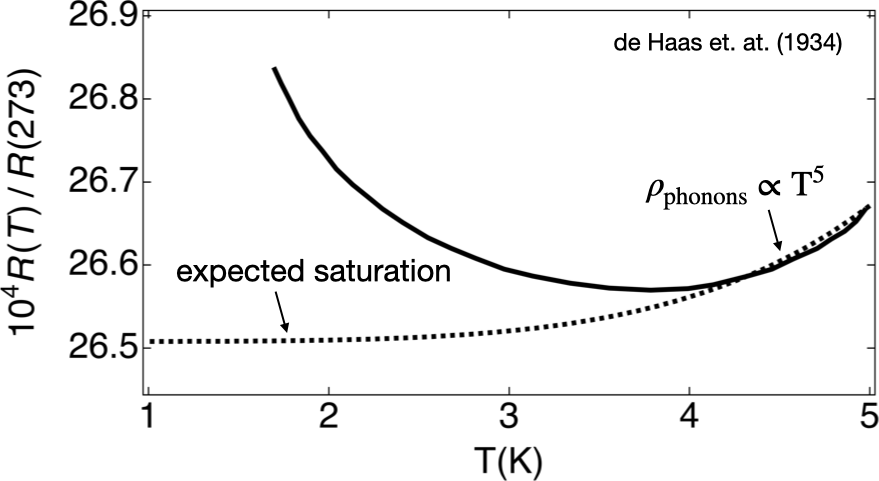
\includegraphics[width=0.9\textwidth]{figures/ch2/crop_FiguresMaster.008.png}
  \caption[Kondo effect in bulk materials]{\label{fig:ch2/kondo_bulkmetal} 
  % For some options that work with pdf\LaTeX, please see this discussion:
  %  \url{http://tex.stackexchange.com/questions/11839}. 
  Temperature dependence of the resistivity, $\mathrm{R}$. Due to electron phonon scattering, the resistivity initially decreases as $T^5$. Due to the Kondo effect, the resistivity reaches a minima before it starts increasing logarithmically with decreasing $\mathrm{T}$. The data used for this figure was obtained from~\cite{de_haas}.
   }
 \end{center}
\end{figure}


\begin{figure}[!hbt]
 \begin{center}
%% includegraphics: comment the following if not using the graphicx package
  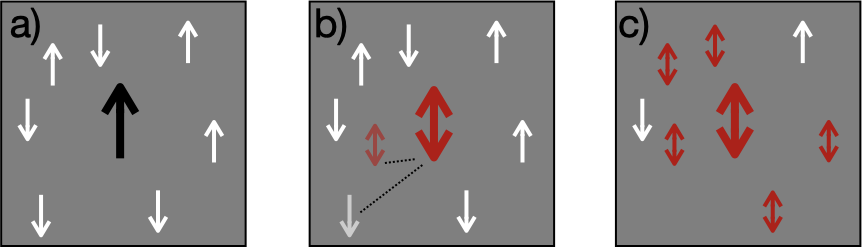
\includegraphics[width=0.9\textwidth]{figures/ch2/crop_FiguresMaster.009.png}
  \caption[Kondo effect illustration]{\label{fig:ch2/kondo_bulkdiagram} 
  % For some options that work with pdf\LaTeX, please see this discussion:
  %  \url{http://tex.stackexchange.com/questions/11839}. 
  (\textbf{a}) A single magnetic impurity (black arrow) is surrounded by conduction electrons (white arrow). (\textbf{b}) Conduction electrons scatter off the magnetic impurity resulting in a possible spin flip of both particles. This leaves the particles entangled. (\textbf{c}) Continued scattering events build a macroscopic coherent state known as a `Kondo singlet' .
   }
 \end{center}
\end{figure}


It took until 1964 for a theoretical explanation of the resistivity minima~\cite{jun_kondo}. Jun Kondo used the s-d model, which couples a metal (non-magnetic, s-band) to a magnetic impurity (un filled d-level). By looking at higher order contributions to the resistivity, a logarithmic term appears, resulting in a large correction at low $\mathrm{T}$. This contribution come from a processes where spin exchange interactions occur. This work showed that a magnetic impurity at low temperatures can give rise to an alternative scattering process, involving a temporary exchange of spin states between the magnetic impurity and surrounding conduction electrons. Fig.~\ref{fig:ch2/kondo_bulkdiagram} illustrates how exchange of spin states can build up a coherent state between the magnetic impurity and the free conduction electrons. It begins with Fig.~\ref{fig:ch2/kondo_bulkdiagram}\textbf{a} where a magnetic impurity is surrounded by conduction electrons. 
Fig.~\ref{fig:ch2/kondo_bulkdiagram}\textbf{b} shows a scattering event which may, or may not result in the spin flip of the conduction electron and the magnetic impurity. This leaves the two particles entangled. Continued scattering events between the magnetic impurity and conduction electrons will result in a macroscopic state Fig.~\ref{fig:ch2/kondo_bulkdiagram}\textbf{c}. This is known as a `Kondo singlet' or `Kondo cloud'. It is found that only a single parameter is needed to describe the low temperature properties and formation of the Kondo singlet, the Kondo temperature $\mathrm{T_k}$. Further discussion on the theory of the Kondo effect is out of the scope of this thesis but an excellent summary is found here~\cite{kondo_theory_history}. 




\afterpage{\clearpage}
\section{Kondo Effect in Quantum Dots}

\begin{figure}[!hbt]
 \begin{center}
%% includegraphics: comment the following if not using the graphicx package
  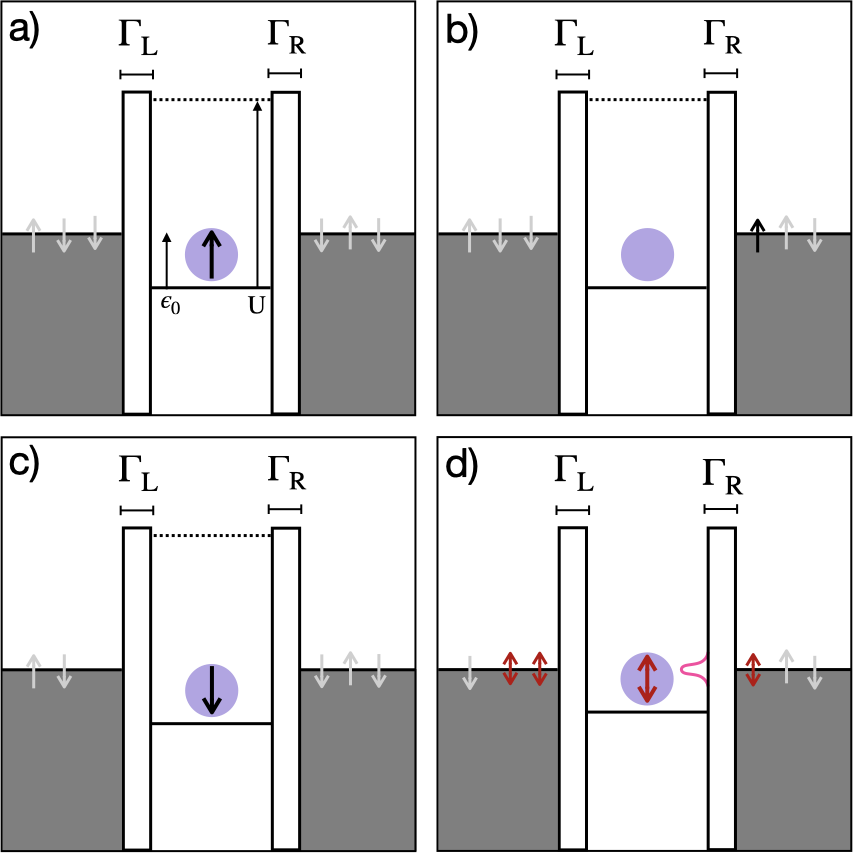
\includegraphics[width=0.75\textwidth]{figures/ch2/crop_FiguresMaster.010.png}
  \caption[Kondo effect in a quantum dot: Coulomb blockade energy diagrams]{\label{fig:ch2/kondo_dot_diagram} 
  % For some options that work with pdf\LaTeX, please see this discussion:
  %  \url{http://tex.stackexchange.com/questions/11839}. 
  A Coulomb blockade energy diagram illustrating the formation of a Kondo singlet in a quantum dot. Here the dot acts as a localised spin. The dark grey represents the continuous energy level of electrons in the leads. The white rectangles represent tunnel barriers between the quantum dot and leads. The rate of tunneling is denoted by the parameter $\Gamma$, the wider (narrower) the barrier, the smaller (larger) the rate of tunneling. (\textbf{a}) The quantum dot has a one spin degenerate energy level with dot energy $\mathrm{\epsilon_0}$, occupied by a single electron. The next energy level is separated by the charging energy, $\mathrm{U}$. In Figure~\ref{fig:ch1/dot_intro} zero conductance is expected through the quantum dot. However, (\textbf{b},\textbf{c}) depict a possible virtual tunneling event, where the spin up electron tunnels out of the dot and a spin down electron tunnels into the dot within a short time. (\textbf{d}) shows how virtual tunnel events involving possible spin flips lead to a correlated state, the Kondo singlet. This state is pictured as a narrow density of states formed at the Fermi energy of the leads. If a Kondo singlet has been formed, enhanced conductance is measured though the quantum dot, even as the dot energy $\epsilon_0$ is below the energy level of the leads. Note the formation of the Kondo singlet requires an odd number of electrons in the quantum dot.
   }
 \end{center}
\end{figure}


Until the late 1990s, the Kondo effect had been primarily explored by theorists, due to the difficulty of experimentally controlling the Kondo state~\cite{kondo_review}. However, after advances in quantum dot design, the potential for precise in situ control was irresistible and the first measurement of a Kondo singlet was in 1998~\cite{goldhaber_first_kondo}. It was also around this time, that scanning tunnelling microscope (STM) was used to study the Kondo effect~\cite{stm_kondo}.

In quantum dots, an odd number of electrons results in an unpaired electron that acts as the magnetic impurity in bulk metals. Similar to bulk metals, the conduction electrons in the 2DEG can interact with the net spin in the quantum dot. The advantage of studying the Kondo effect in quantum dots comes from the in situ control over the coupling strength, voltage bias, and energy level of the magnetic impurity.

The formation of a Kondo singlet in quantum dots can be illustrated similarly to that in bulk metals Fig.~\ref{fig:ch2/kondo_dot_diagram}. 
If the dot energy of the quantum dot is far below the Fermi energy of the leads, the electron is not expected to tunnel out of the dot as it does not have the required energy to reach the available empty energy levels in the leads. However, a second order tunnelling process can occur where the electron in the dot tunnels into the leads Fig.~\ref{fig:ch2/kondo_dot_diagram}\textbf{b}, as long as another electron tunnels into the quantum dot within the timescale limited by Heisenberg’s uncertainty principle Fig.~\ref{fig:ch2/kondo_dot_diagram}\textbf{c}. This second order process can result in a spin flip of the impurity. Many of these virtual tunneling events will lead to the formation of a singlet state, resulting in a narrow density of states formed at the Fermi energy of the leads Fig.~\ref{fig:ch2/kondo_dot_diagram}\textbf{d}. 


 \begin{figure}[!hbt]
 \begin{center}
%% includegraphics: comment the following if not using the graphicx package
  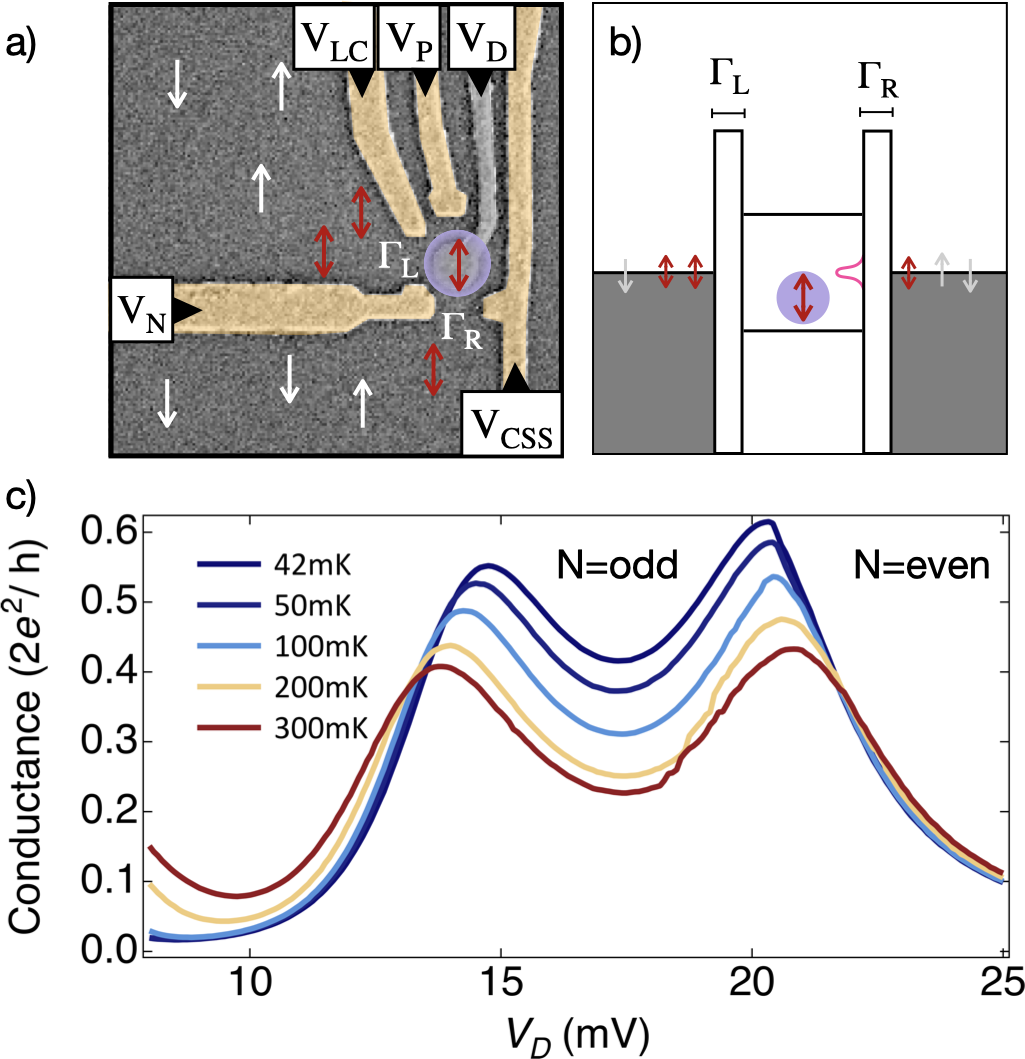
\includegraphics[width=0.9\textwidth]{figures/ch2/crop_FiguresMaster.011.png}
  \caption[Kondo effect in a quantum dot in the Kondo regime]{\label{fig:ch2/kondo_regime_conductance} 
  % For some options that work with pdf\LaTeX, please see this discussion:
  %  \url{http://tex.stackexchange.com/questions/11839}. 
  (\textbf{a}) An SEM image of the gates used to define a quantum dot. The dot contains an odd number of electrons and the tunnel barriers are tuned so that a Kondo singlet is formed. (\textbf{b}) A Coulomb blockade energy diagram picture of a Kondo singlet. As the dot energy falls below the energy level of the leads, there is enhanced conductance due to virtual tunneling events through the quantum dot. (\textbf{c}) Data showing the temperature dependence of conductance through a quantum dot when a Kondo singlet is formed. In the even occupied sides conductance decreases as the temperature is lowered. On odd occupation, a Kondo singlet forms and conductance increases with decreasing temperature.}
 \end{center}
\end{figure}



 Unlike the resistivity increase in bulk metals, the presence of a Kondo singlet leads to enhanced conductance through the quantum dot Fig.~\ref{fig:ch2/kondo_regime_conductance}. The enhanced conductance increases, as the system temperature fall below the Kondo temperature $\mathrm{T_k}$. Similar to bulk metals, the existence of the Kondo effect in quantum dots requires the system temperature being lower than the Kondo temperature $\mathrm{T_k}$. 

\begin{equation}\label{eq:kondo_temp}
 \mathrm{T_K} = 
 \frac{\sqrt{\Gamma \mathrm{U}}}{2}
 e^{\pi \epsilon_0 (\epsilon_0 + \mathrm{U})/\Gamma\mathrm{U}}
\end{equation}

where $\Gamma$ is the coupling from both source and drain leads, $\mathrm{\Gamma = \Gamma_L + \Gamma_R}$. When the dot energy is far below the Fermi level in the leads (i.e. the full charge of the un paired electron is in the quantum dot), the Kondo temperature depends exponentially on the depth of the dot energy~\cite{goldhaber_mv}. The Kondo temperature also depends on the strength of coupling i.e. the stronger the coupling, the larger the Kondo temperature. This expression for the Kondo temperature only holds in the `Kondo regime'. The Kondo regime is characterised by $\tilde{\epsilon}_0<<-0.5$ where $\tilde{\epsilon}\equiv \epsilon_0/\Gamma$. Qualitatively, this regime is satisfied when the full charge of the electron is in the quantum dot. Consequently, as the dot energy is raised so that only a fraction of the electron charge is localised in the quantum dot, this expression for the Kondo temperature breaks down. However, the quantum dot still exhibits a net spin and Kondo enhancement remains present. Importantly, the Kondo temperature increases as the dot energy approaches the Fermi energy of the leads~\cite{goldhaber_mv}, although it may not be exponential in form. 

Many of the early measurements on the Kondo effect in quantum dots used very strong couplings so the system temperature remained below the Kondo temperature deep into the Kondo regime~\cite{kondo_unitary}. Such studies examined temperature dependence of the conductance in the Coulomb blockade valley where the conductance dependence on temperature is non monotonic and has a minimum at finite temperatures~\cite{Pustilnik2004}. It was found that in the Kondo regime, the Kondo temperature Eq.~\ref{eq:kondo_temp} sets a new many body scale. The Kondo temperature can be used to normalise the conductance such that it is independent of other energy scales $\Gamma$, $\mathrm{U}$ and $\tilde{\epsilon}_0$.

\begin{equation}\label{eq:kondo_conductance}
 \mathrm{G(T)} =
 \mathrm{G_0}
 \left(
 \frac{\mathrm{T_k'^{2}}}{\mathrm{T^2} + \mathrm{T_k'^{2}}}
 \right)^\mathrm{s}
\end{equation}

where $\mathrm{T_k'^{2}} = \mathrm{T_k}/\sqrt{2^{\mathrm{1/s}}-1}$ and $\mathrm{s} \approx 0.20$ for a spin 1/2 system in the Kondo regime~\cite{goldhaber_mv}. The parameter $\mathrm{s}$ determines the steepness of the conductance drop with increasing temperature. The one parameter scaling of the conductance in the Kondo regime is used as one of the demonstrations of the Kondo effect. Other measurements include a zero bias peak in the Coulomb blockade valley~\cite{kondo_unitary} and a splitting of this zero bias peak with magnetic field~\cite{cronenwett_tunable_kondo}. 

Other efforts have been made to explore the Kondo effect with less strong coupling. In this regime, the conductance in the middle of the Coulomb blockade valley does not follow the surprising increase with decreasing temperature~\cite{goldhaber_mv}. However, the Kondo temperature increases as the dot energy approaches the Fermi energy of the leads and a conductance enhancement can be recovered at sufficiently low system temperatures. This regime of weaker coupling is the focus of the next chapter. 


